% !TEX root = ../main.tex
\section{Results}
\label{sec:results}

\subsection{Depth encoder}
\label{sec:results-encoder}
% source: uuv-rl-env (worktree environment) experiments/logs/dce_train_{25888723,25888960,25903576}.out,
%         encoder/datasets.md, encoder/docs/dce_D001_box_recon.png
The depth encoder of Section~\ref{sec:depth-encoder} was trained on the 90,221 training images of the dataset and evaluated on the 9,700 validation images. Three runs were made (Table~\ref{tab:dce-results}). The first two use the original collision image of \textcite{kulkarni2023task}, with a cube of half-edge \SI{0.3}{\metre} as the robot; the second continues the first for 150 more epochs with a restarted learning rate. The final run uses the box-shaped robot of Section~\ref{sec:depth-encoder}, which is closer to the shape of the vehicle, and is the encoder used by the policy.

\begin{table}[ht]
\centering
\caption{Training runs of the depth encoder on the validation set, at the epoch with the lowest validation loss. The loss is the per-image sum of squared errors of the collision image (normalised to $[0,1]$) plus the KL term; the RMSE is the reconstruction error in metres. The two targets differ, so their errors are only roughly comparable.}
\label{tab:dce-results}
\begin{tabular}{@{}lrrrrrr@{}}
\toprule
Target & Epochs & Best epoch & Loss & Reconstruction & KL & RMSE (\si{\metre}) \\
\midrule
Cube                & 100 & 100 & 55.83 & 33.65 & 22.17 & 0.604 \\
Cube, resumed       & 250 & 248 & 52.05 & 30.64 & 21.41 & 0.577 \\
Box (final)         & 250 & 244 & 52.37 & 28.94 & 23.43 & 0.560 \\
\bottomrule
\end{tabular}
\end{table}

The validation error falls quickly in the first 50 epochs and levels out at around \SI{0.56}{\metre} (Figure~\ref{fig:dce-curve}). The box target gives the lowest reconstruction error, although its KL term is higher, meaning that the latent carries slightly more information. Training the final run took about \SI{30}{\minute} on one GPU.

\begin{figure}[ht]
    \centering
    % !TEX root = ../main.tex
% Validation RMSE of the depth encoder (DCE) per epoch, bb_theme palette.
% GENERATED by scripts/make_dce_curve.py from the uuv-rl-env training logs; do not edit by hand.
% x: 0.04 cm per epoch; y: 5 cm per metre, from 0.4 m.
% Use inside a figure environment:  % !TEX root = ../main.tex
% Validation RMSE of the depth encoder (DCE) per epoch, bb_theme palette.
% GENERATED by scripts/make_dce_curve.py from the uuv-rl-env training logs; do not edit by hand.
% x: 0.04 cm per epoch; y: 5 cm per metre, from 0.4 m.
% Use inside a figure environment:  % !TEX root = ../main.tex
% Validation RMSE of the depth encoder (DCE) per epoch, bb_theme palette.
% GENERATED by scripts/make_dce_curve.py from the uuv-rl-env training logs; do not edit by hand.
% x: 0.04 cm per epoch; y: 5 cm per metre, from 0.4 m.
% Use inside a figure environment:  \input{figures/dce-curve.tex}
\definecolor{vaeInk}{HTML}{0F1B2D}
\definecolor{vaeSignal}{HTML}{1D5FD1}
\definecolor{vaeMuted}{HTML}{56677F}
\definecolor{vaeHatch}{HTML}{2F3FD0}
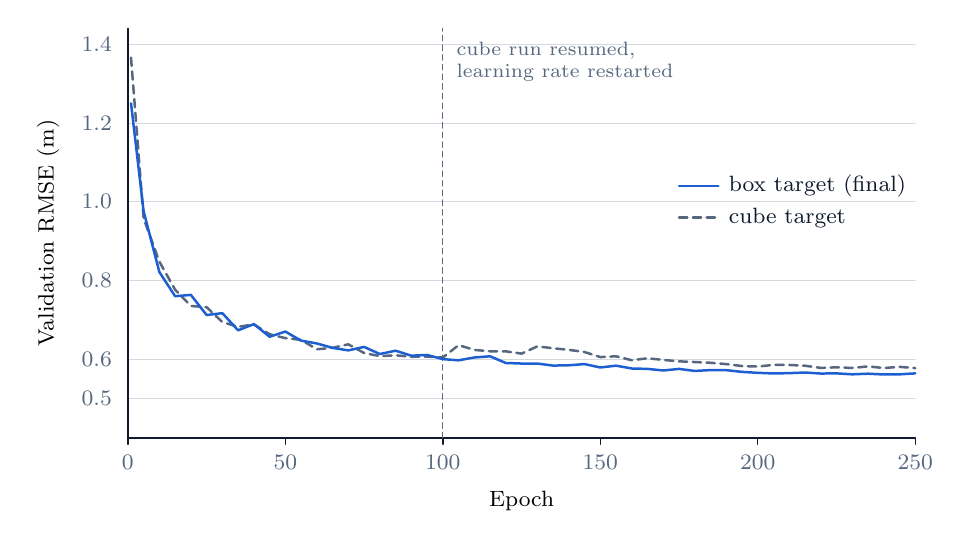
\begin{tikzpicture}[font=\footnotesize, line cap=round, line join=round]
  % grid and axes
  \foreach \y/\l in {0.5/0.5, 1/0.6, 2/0.8, 3/1.0, 4/1.2, 5/1.4} {
    \draw[vaeMuted!25, line width=0.3pt] (0,\y) -- (10,\y);
    \node[anchor=east, text=vaeMuted] at (-0.08,\y) {\l};
  }
  \foreach \x/\l in {0/0, 2/50, 4/100, 6/150, 8/200, 10/250} {
    \draw[vaeInk, line width=0.5pt] (\x,0) -- (\x,-0.08);
    \node[anchor=north, text=vaeMuted] at (\x,-0.1) {\l};
  }
  \draw[vaeInk, line width=0.6pt] (0,0) -- (10,0);
  \draw[vaeInk, line width=0.6pt] (0,0) -- (0,5.2);
  \node[anchor=north] at (5,-0.55) {Epoch};
  \node[rotate=90, anchor=south] at (-0.75,2.6) {Validation RMSE (m)};
  % resume of the cube run
  \draw[vaeMuted, line width=0.4pt, dash pattern=on 2pt off 1.5pt] (4,0) -- (4,5.2);
  \node[anchor=north west, text=vaeMuted, font=\scriptsize, align=left] at (4.05,5.15) {cube run resumed,\\learning rate restarted};
  % curves
  \draw[vaeMuted, line width=0.9pt, dash pattern=on 3pt off 2pt] plot coordinates {(0.04,4.830) (0.20,2.788) (0.40,2.239) (0.60,1.883) (0.80,1.676) (1.00,1.661) (1.20,1.472) (1.40,1.411) (1.60,1.442) (1.80,1.317) (2.00,1.268) (2.20,1.246) (2.40,1.126) (2.60,1.145) (2.80,1.189) (3.00,1.079) (3.20,1.039) (3.40,1.050) (3.60,1.031) (3.80,1.033) (4.00,1.021) (4.20,1.179) (4.40,1.118) (4.60,1.101) (4.80,1.100) (5.00,1.071) (5.20,1.163) (5.40,1.139) (5.60,1.119) (5.80,1.091) (6.00,1.027) (6.20,1.037) (6.40,0.987) (6.60,1.012) (6.80,0.991) (7.00,0.973) (7.20,0.964) (7.40,0.955) (7.60,0.938) (7.80,0.913) (8.00,0.907) (8.20,0.928) (8.40,0.927) (8.60,0.917) (8.80,0.890) (9.00,0.897) (9.20,0.889) (9.40,0.909) (9.60,0.888) (9.80,0.903) (10.00,0.887)};
  \draw[vaeSignal, line width=0.9pt] plot coordinates {(0.04,4.250) (0.20,2.879) (0.40,2.107) (0.60,1.800) (0.80,1.817) (1.00,1.561) (1.20,1.585) (1.40,1.367) (1.60,1.446) (1.80,1.285) (2.00,1.351) (2.20,1.236) (2.40,1.200) (2.60,1.144) (2.80,1.112) (3.00,1.156) (3.20,1.066) (3.40,1.108) (3.60,1.045) (3.80,1.054) (4.00,1.001) (4.20,0.986) (4.40,1.022) (4.60,1.037) (4.80,0.952) (5.00,0.945) (5.20,0.945) (5.40,0.919) (5.60,0.923) (5.80,0.938) (6.00,0.895) (6.20,0.918) (6.40,0.882) (6.60,0.877) (6.80,0.857) (7.00,0.877) (7.20,0.851) (7.40,0.862) (7.60,0.861) (7.80,0.839) (8.00,0.827) (8.20,0.819) (8.40,0.823) (8.60,0.831) (8.80,0.818) (9.00,0.820) (9.20,0.808) (9.40,0.816) (9.60,0.806) (9.80,0.808) (10.00,0.820)};
  % legend
  \draw[vaeSignal, line width=0.9pt] (7.0,3.2) -- (7.5,3.2) node[anchor=west, text=vaeInk] {box target (final)};
  \draw[vaeMuted, line width=0.9pt, dash pattern=on 3pt off 2pt] (7.0,2.8) -- (7.5,2.8) node[anchor=west, text=vaeInk] {cube target};
\end{tikzpicture}

\definecolor{vaeInk}{HTML}{0F1B2D}
\definecolor{vaeSignal}{HTML}{1D5FD1}
\definecolor{vaeMuted}{HTML}{56677F}
\definecolor{vaeHatch}{HTML}{2F3FD0}
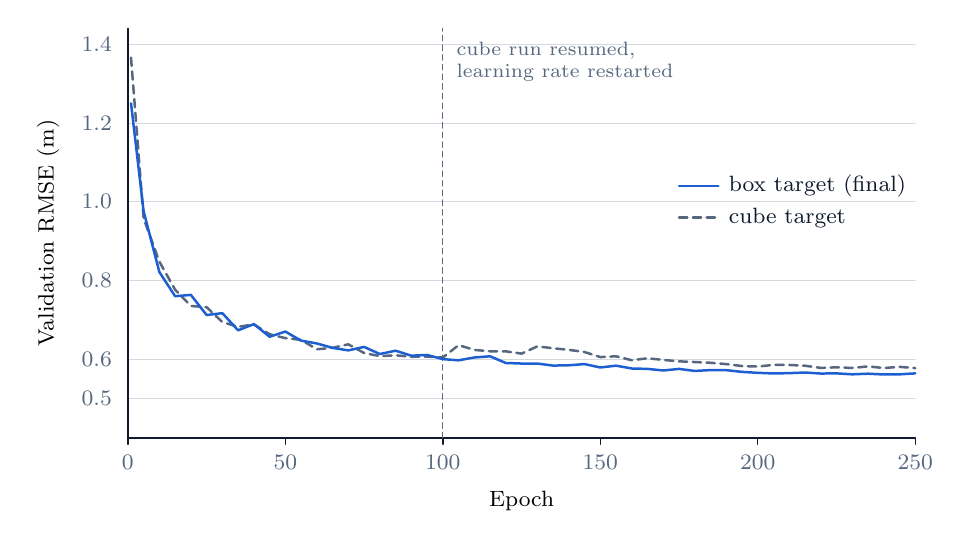
\begin{tikzpicture}[font=\footnotesize, line cap=round, line join=round]
  % grid and axes
  \foreach \y/\l in {0.5/0.5, 1/0.6, 2/0.8, 3/1.0, 4/1.2, 5/1.4} {
    \draw[vaeMuted!25, line width=0.3pt] (0,\y) -- (10,\y);
    \node[anchor=east, text=vaeMuted] at (-0.08,\y) {\l};
  }
  \foreach \x/\l in {0/0, 2/50, 4/100, 6/150, 8/200, 10/250} {
    \draw[vaeInk, line width=0.5pt] (\x,0) -- (\x,-0.08);
    \node[anchor=north, text=vaeMuted] at (\x,-0.1) {\l};
  }
  \draw[vaeInk, line width=0.6pt] (0,0) -- (10,0);
  \draw[vaeInk, line width=0.6pt] (0,0) -- (0,5.2);
  \node[anchor=north] at (5,-0.55) {Epoch};
  \node[rotate=90, anchor=south] at (-0.75,2.6) {Validation RMSE (m)};
  % resume of the cube run
  \draw[vaeMuted, line width=0.4pt, dash pattern=on 2pt off 1.5pt] (4,0) -- (4,5.2);
  \node[anchor=north west, text=vaeMuted, font=\scriptsize, align=left] at (4.05,5.15) {cube run resumed,\\learning rate restarted};
  % curves
  \draw[vaeMuted, line width=0.9pt, dash pattern=on 3pt off 2pt] plot coordinates {(0.04,4.830) (0.20,2.788) (0.40,2.239) (0.60,1.883) (0.80,1.676) (1.00,1.661) (1.20,1.472) (1.40,1.411) (1.60,1.442) (1.80,1.317) (2.00,1.268) (2.20,1.246) (2.40,1.126) (2.60,1.145) (2.80,1.189) (3.00,1.079) (3.20,1.039) (3.40,1.050) (3.60,1.031) (3.80,1.033) (4.00,1.021) (4.20,1.179) (4.40,1.118) (4.60,1.101) (4.80,1.100) (5.00,1.071) (5.20,1.163) (5.40,1.139) (5.60,1.119) (5.80,1.091) (6.00,1.027) (6.20,1.037) (6.40,0.987) (6.60,1.012) (6.80,0.991) (7.00,0.973) (7.20,0.964) (7.40,0.955) (7.60,0.938) (7.80,0.913) (8.00,0.907) (8.20,0.928) (8.40,0.927) (8.60,0.917) (8.80,0.890) (9.00,0.897) (9.20,0.889) (9.40,0.909) (9.60,0.888) (9.80,0.903) (10.00,0.887)};
  \draw[vaeSignal, line width=0.9pt] plot coordinates {(0.04,4.250) (0.20,2.879) (0.40,2.107) (0.60,1.800) (0.80,1.817) (1.00,1.561) (1.20,1.585) (1.40,1.367) (1.60,1.446) (1.80,1.285) (2.00,1.351) (2.20,1.236) (2.40,1.200) (2.60,1.144) (2.80,1.112) (3.00,1.156) (3.20,1.066) (3.40,1.108) (3.60,1.045) (3.80,1.054) (4.00,1.001) (4.20,0.986) (4.40,1.022) (4.60,1.037) (4.80,0.952) (5.00,0.945) (5.20,0.945) (5.40,0.919) (5.60,0.923) (5.80,0.938) (6.00,0.895) (6.20,0.918) (6.40,0.882) (6.60,0.877) (6.80,0.857) (7.00,0.877) (7.20,0.851) (7.40,0.862) (7.60,0.861) (7.80,0.839) (8.00,0.827) (8.20,0.819) (8.40,0.823) (8.60,0.831) (8.80,0.818) (9.00,0.820) (9.20,0.808) (9.40,0.816) (9.60,0.806) (9.80,0.808) (10.00,0.820)};
  % legend
  \draw[vaeSignal, line width=0.9pt] (7.0,3.2) -- (7.5,3.2) node[anchor=west, text=vaeInk] {box target (final)};
  \draw[vaeMuted, line width=0.9pt, dash pattern=on 3pt off 2pt] (7.0,2.8) -- (7.5,2.8) node[anchor=west, text=vaeInk] {cube target};
\end{tikzpicture}

\definecolor{vaeInk}{HTML}{0F1B2D}
\definecolor{vaeSignal}{HTML}{1D5FD1}
\definecolor{vaeMuted}{HTML}{56677F}
\definecolor{vaeHatch}{HTML}{2F3FD0}
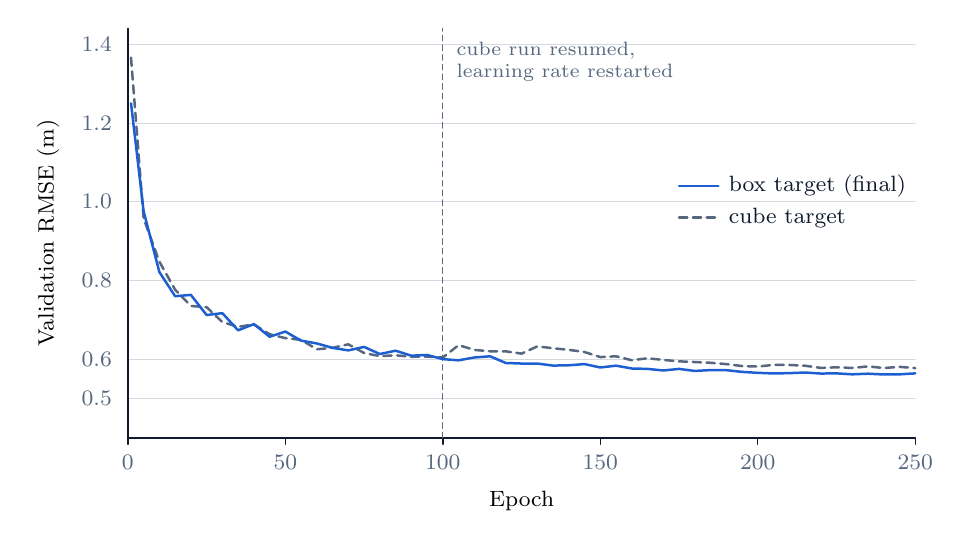
\begin{tikzpicture}[font=\footnotesize, line cap=round, line join=round]
  % grid and axes
  \foreach \y/\l in {0.5/0.5, 1/0.6, 2/0.8, 3/1.0, 4/1.2, 5/1.4} {
    \draw[vaeMuted!25, line width=0.3pt] (0,\y) -- (10,\y);
    \node[anchor=east, text=vaeMuted] at (-0.08,\y) {\l};
  }
  \foreach \x/\l in {0/0, 2/50, 4/100, 6/150, 8/200, 10/250} {
    \draw[vaeInk, line width=0.5pt] (\x,0) -- (\x,-0.08);
    \node[anchor=north, text=vaeMuted] at (\x,-0.1) {\l};
  }
  \draw[vaeInk, line width=0.6pt] (0,0) -- (10,0);
  \draw[vaeInk, line width=0.6pt] (0,0) -- (0,5.2);
  \node[anchor=north] at (5,-0.55) {Epoch};
  \node[rotate=90, anchor=south] at (-0.75,2.6) {Validation RMSE (m)};
  % resume of the cube run
  \draw[vaeMuted, line width=0.4pt, dash pattern=on 2pt off 1.5pt] (4,0) -- (4,5.2);
  \node[anchor=north west, text=vaeMuted, font=\scriptsize, align=left] at (4.05,5.15) {cube run resumed,\\learning rate restarted};
  % curves
  \draw[vaeMuted, line width=0.9pt, dash pattern=on 3pt off 2pt] plot coordinates {(0.04,4.830) (0.20,2.788) (0.40,2.239) (0.60,1.883) (0.80,1.676) (1.00,1.661) (1.20,1.472) (1.40,1.411) (1.60,1.442) (1.80,1.317) (2.00,1.268) (2.20,1.246) (2.40,1.126) (2.60,1.145) (2.80,1.189) (3.00,1.079) (3.20,1.039) (3.40,1.050) (3.60,1.031) (3.80,1.033) (4.00,1.021) (4.20,1.179) (4.40,1.118) (4.60,1.101) (4.80,1.100) (5.00,1.071) (5.20,1.163) (5.40,1.139) (5.60,1.119) (5.80,1.091) (6.00,1.027) (6.20,1.037) (6.40,0.987) (6.60,1.012) (6.80,0.991) (7.00,0.973) (7.20,0.964) (7.40,0.955) (7.60,0.938) (7.80,0.913) (8.00,0.907) (8.20,0.928) (8.40,0.927) (8.60,0.917) (8.80,0.890) (9.00,0.897) (9.20,0.889) (9.40,0.909) (9.60,0.888) (9.80,0.903) (10.00,0.887)};
  \draw[vaeSignal, line width=0.9pt] plot coordinates {(0.04,4.250) (0.20,2.879) (0.40,2.107) (0.60,1.800) (0.80,1.817) (1.00,1.561) (1.20,1.585) (1.40,1.367) (1.60,1.446) (1.80,1.285) (2.00,1.351) (2.20,1.236) (2.40,1.200) (2.60,1.144) (2.80,1.112) (3.00,1.156) (3.20,1.066) (3.40,1.108) (3.60,1.045) (3.80,1.054) (4.00,1.001) (4.20,0.986) (4.40,1.022) (4.60,1.037) (4.80,0.952) (5.00,0.945) (5.20,0.945) (5.40,0.919) (5.60,0.923) (5.80,0.938) (6.00,0.895) (6.20,0.918) (6.40,0.882) (6.60,0.877) (6.80,0.857) (7.00,0.877) (7.20,0.851) (7.40,0.862) (7.60,0.861) (7.80,0.839) (8.00,0.827) (8.20,0.819) (8.40,0.823) (8.60,0.831) (8.80,0.818) (9.00,0.820) (9.20,0.808) (9.40,0.816) (9.60,0.806) (9.80,0.808) (10.00,0.820)};
  % legend
  \draw[vaeSignal, line width=0.9pt] (7.0,3.2) -- (7.5,3.2) node[anchor=west, text=vaeInk] {box target (final)};
  \draw[vaeMuted, line width=0.9pt, dash pattern=on 3pt off 2pt] (7.0,2.8) -- (7.5,2.8) node[anchor=west, text=vaeInk] {cube target};
\end{tikzpicture}

    \caption{Validation RMSE of the depth encoder per epoch. The cube run was resumed after 100 epochs with a restarted learning rate.}
    \label{fig:dce-curve}
\end{figure}

Figure~\ref{fig:dce-recon} shows the final encoder on six validation images. The target in the second column differs visibly from the depth image in the first, because it is not the depth image but the collision image $D^{\mathrm{col}}_t$ of Section~\ref{sec:depth-encoder}: for each pixel, the distance the vehicle can travel along that pixel's ray before its body touches a surface. Every range is therefore shortened by the size of the vehicle, and obstacles grow sideways by about its half-width, so that the target always lies at or below the depth image. When the camera is close to a surface, nearly the whole image is within the vehicle's size of it, and the collision image is close to zero everywhere, as in the fourth and fifth rows, even though the depth image still shows structure further away. Open space and the outlines of the inflated obstacles are reconstructed. The decoded images are smoother than the targets: the largest errors are at sharp edges, such as the boundary between an obstacle and open water. Views taken close to an obstacle, where almost the whole collision image is near zero, are reconstructed with an error of about \SI{0.1}{\metre}.

\begin{figure}[ht]
    \centering
    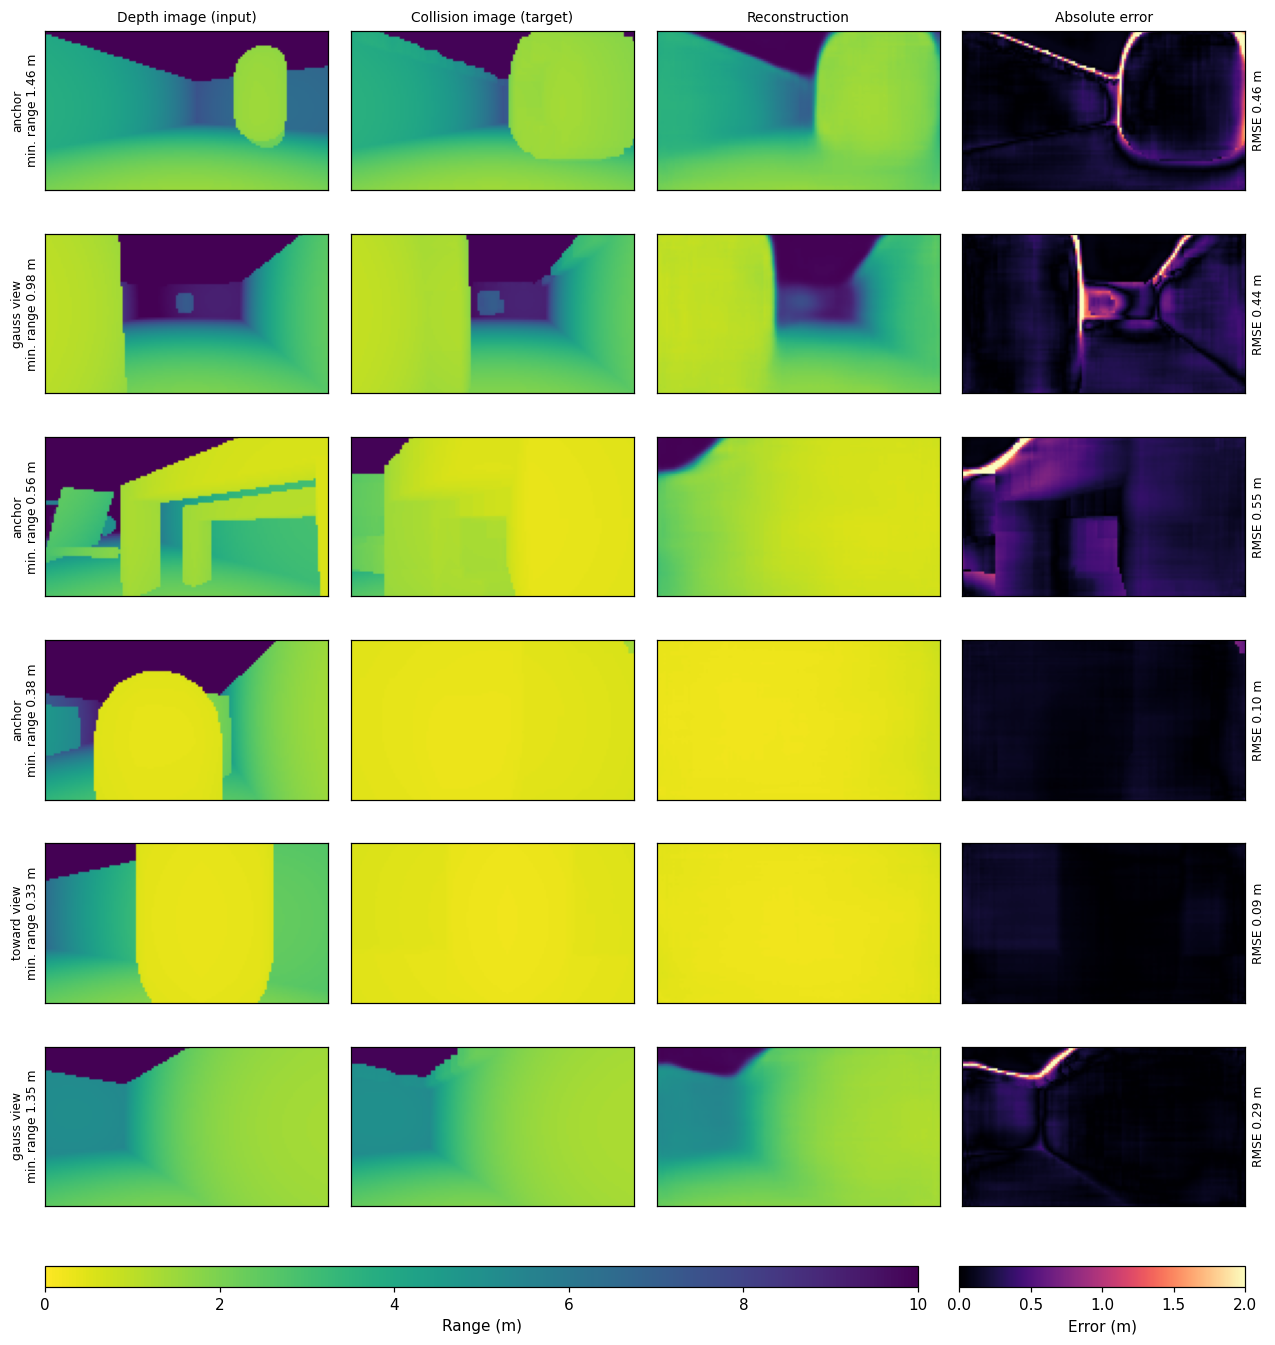
\includegraphics[width=\linewidth]{figures/dce_recon.png}
    \caption{Final depth encoder (best epoch) on six validation images with clean input. Columns: the depth image given to the encoder, the collision image it is trained to reconstruct, the reconstruction and the absolute error, with the RMSE of each image on the right. Each row is labelled on the left with its kind and the minimum range in the depth image: an anchor is a view from the policy rollout, a Gaussian view is taken from a randomly perturbed camera pose, and a toward view from a pose moved along the shortest sonar ray, facing the nearest obstacle.}
    \label{fig:dce-recon}
\end{figure}

\begin{todolist}
  \item Policy training results (success rate, collisions) and the memory comparison of RQ3.
\end{todolist}
\subsection{Quantitative Results}

\subsection{Qualitative Results}

\subsection{Ablation Study}

% Place all Results figures before the Discussion (the reconstruction figure otherwise
% floats past the bibliography into the appendix).
\clearpage
